\section{Tema 4. Medidas de tensiones, intensidades y resistencias.}
\subsection{Métodos industriales frente a métodos de laboratorio.}
\begin{itemize}
	\item \textbf{Métodos industriales:}
	\begin{itemize}
		\item Utilizan aparatos de medida básicos.
		\item No es necesaria formación especial.
		\item No son muy exactos, pero tienen precisión suficiente.
		\item Dan respuestas inmediatas.
	\end{itemize}
	\item \textbf{Métodos de laboratorio:}
	\begin{itemize}
		\item Requieren equipos de gran calidad metrológica.
		\item Los operadores deben ser capacitados para su uso.
		\item Las tomas de datos se realizan bajo condiciones controladas.
		\item Buscan minimizar la incertidumbre de medida.
	\end{itemize}
\end{itemize}


\subsection{Métodos industriales para medir tensión e intensidad.}
Para un buen resultado se debe prestar atención a:
\begin{itemize}
	\item La selección adecuada de los campos de medida.
	\item La clase del aparato y su error de inserción.
	\item Si el aparato mide el verdadero valor eficaz.
	\item La posición de empleo.
	\item Las condiciones ambientales.
	\item El ancho de banda.
\end{itemize}
\subsection{Error de inserción.}
Debido a la resistencia interna de los aparatos un voltímetro indica una tensión menor a la medida y el amperímetro una corriente menor a la medida. Como los circuitos equivalentes de un voltímetro y amperímetro son:

\begin{itemize}
	\item En voltímetros:
	\begin{itemize}
		\item Es importante que $R << R_V$
	\end{itemize}
	\item En amperímetros:
	\begin{itemize}
		\item Es importante que $R_A << R$
	\end{itemize}
\end{itemize}


\begin{figure}[H]
	\centering
	\begin{circuitikz}
		\tikzstyle{every node}=[font=\normalsize]
		\draw (5.75,13) to[R,l={ \normalsize R}] (5.75,16.25);
		\draw (7.25,14.5) to[rmeter, t=V] (7.25,13);
		\draw (7.25,16.25) to[R,l={ \normalsize $R_v$}] (7.25,14.5);
		\draw [](5.75,16.25) to[short] (7.25,16.25);
		\draw [](5.75,13) to[short] (7.25,13);
		\node at (6.5,16.25) [circ] {};
		\node at (6.5,13) [circ] {};
		\draw [](6.5,16.25) to[short, -o] (6.5,16.75) ;
		\draw [](6.5,12.5) to[short, o-] (6.5,13) ;
		\draw (10,17.25) to[R,l={ \normalsize $R_A$}] (10,15.25);
		\draw (10,15.25) to[rmeter, t=A] (10,14);
		\draw (10,14) to[R,l={ \normalsize $R$}] (10,12);
		\draw [](10,17.25) to[short, -o] (10,17.5) ;
		\draw [](10,11.75) to[short, o-] (10,12) ;
	\end{circuitikz}
	
	\label{fig:2}
\end{figure}

\subsubsection{Medida de tensión en circuitos de alta impedancia.}
La conexión de un voltímetro a un circuito de alta impedancia puede producir una reducción importante en la tensión a medir. Para ello, se realiza la siguiente comprobación:

\begin{enumerate}
	\item Se mide la tensión deseada con un voltímetro $U_1$.
	\item Se coloca una resistencia ajustable $R_s$ en serie con el voltímetro y se ajusta hasta que el voltímetro indica una tensión $U_2=\frac{U_1}{2}$.
	\item En función de los valores obtenidos se pueden obtener 2 conclusiones:
	\begin{enumerate}
		\item Si el valor de $R_s$ es igual a $R_V$ la medida no se ve afectada por la inserción del voltímetro.
		\item Si el valor de $R_s$ es mayor a $R_V$ existe efecto de carga y se realiza la siguiente corrección:
		\[U=U_1\frac{R_s}{R_V}\]   
	\end{enumerate}
\end{enumerate}


\subsection{Medida de resistencia con óhmetros.}
\subsubsection{Digitales.}
Su lectura directa es el valor de la resistencia desconocida. Si ese valor es muy reducido, para mejorar el resultado debe restarse la lectura del óhmetro al cortocircuitar los terminales.  El campo de medida elegido debe ser el más próximo al
valor de la resistencia, para que la incertidumbre del
aparato sea mínima y la lectura tenga suficiente resolución.
\subsubsection{Analógicos.}
Hay que hacer un ajuste de cero inicial y cambiar de campo
para que la aguja quede siempre lo más próxima al centro
de la escala (no es lineal).
\begin{figure}[H]
	\centering
	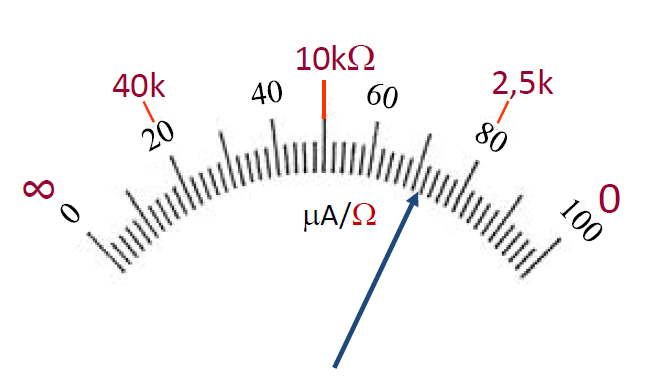
\includegraphics[width=0.5\linewidth]{ImagenesTema4/3}
	\label{fig:3}
\end{figure}



Cabe destacar como la mayor sensibilidad se obtiene cuando la resistencia es nula o igual a la resistencia interna del aparato. Por ello, es mejor medir en la primera mitad de la escala.
\subsection{Medida de resistencia con voltímetro y amperímetro.}
Se mide la corriente y tensión de una carga para obtener la resistencia mediante la ley de Ohm.
\begin{figure}[H]
	\centering
		\begin{circuitikz}[scale = 1.1]
			\tikzstyle{every node}=[font=\normalsize]
			\draw (8,11.5) to[american voltage source] (11.5,11.5);
			\draw (8,12.5) to[rmeter, t=A,l={ \normalsize $R_A$}] (9.75,12.5);
			\draw (11.5,12.5) to[R,l={ \normalsize $R$}] (9.75,12.5);
			\draw (9.75,13.75) to[rmeter, t=V, l={ \normalsize $R_V$}] (11.5,13.75);
			\draw [-latex] (11.5,13.75) -- (11.5,12.5);
			\draw [-latex] (8,13.75) -- (8,12.5);
			\draw [-latex, dashed] (9.75,13.75) -- (9.75,12.5);
			\draw[] (9.75,13.75) to[short] (8,13.75);
			\node at (9.75,12.5) [circ] {};
			\node at (8,12.5) [circ] {};
			\node at (11.5,12.5) [circ] {};
			
			\draw [](8,12.5) to[short] (8,11.5);
			\draw [](11.5,12.5) to[short] (11.5,11.5);
			\node [font=\normalsize] at (8.25,12.75) {A};
			\node [font=\normalsize] at (9.5,12.75) {B};
			\node [font=\normalsize] at (11.75,12.5) {C};
			\node [font=\normalsize] at (7.5,12.5) {$Ml$};
			\node [font=\normalsize] at (9.75,12.25) {$Mc$};
		\end{circuitikz}
	
	\label{fig:my_label}
\end{figure}

En el montaje largo:
\[R'=\frac{U_{AC}}{I_A}=R+R_A\]
\[\epsilon_{ml}=R'-R=R_A \rightarrow \epsilon_{ml(pu)}=\frac{R_A}{R}\]

En el montaje corto:
\[R''=\frac{U_{BC}}{I_A}=\frac{R\cdot R_V}{R+R_V}\]
\[\epsilon_{mc}=-\frac{R^2}{R+R_V} \rightarrow \epsilon_{mc(pu)}=-\frac{R}{R+R_V}\approx-\frac{R}{R_V}\]

Por tanto, para elegir un montaje u otro se igualan los errores y se obtiene el valor crítico:
\[\epsilon_{ml}=\epsilon_{mc}\rightarrow \frac{R_A}{R}\approx\frac{R}{R_V}\rightarrow R_C\approx\sqrt{R_A\cdot R_V}\]
Donde si la resistencia R es mayor a $R_C$ se debe usar el montaje largo y el montaje corto en caso contrario.
\subsection{Medida de R con una $R_p$.}
\subsubsection{Por comparación de corrientes.}
Se mantiene constante $U_0$ y se compara la corriente que circula por la resistencia desconocida y la resistencia patrón.
\begin{figure}[H]
	\begin{minipage}{0.5\textwidth}
		\begin{figure}[H]
			\centering
				\begin{circuitikz}
					\tikzstyle{every node}=[font=\normalsize]
					\draw (10.25,16) to[rmeter, t=A,l={ \normalsize $R_A$}] (12.75,16);
					\draw (10.25,16) to[american voltage source,l={ \normalsize $U_0$}] (10.25,13);
					\draw (12,15) to[R,l={ \normalsize $R_P$}] (12,13);
					\draw (13.5,15) to[R,l={ \normalsize $R_X$}] (13.5,13);
					\draw [](12.75,15.5) to[short, o-] (12.75,16) ;
					\draw [](12,15) to[short, -o] (12.25,15) ;
					\draw [](13.5,15) to[short, -o] (13.25,15) ;
					\draw [-latex] (12.75,15.5) -- (13.25,15);
					\draw[] (13.5,13) to[short] (10.25,13);
					\node at (12,13) [circ] {};
					\draw [-latex] (13.5,15) -- (13.5,14.75)node[pos=0.5,right]{$I_X$};
					\draw [-latex] (12,15) -- (12,14.75)node[pos=0.5,left]{$I_P$};
					\draw [-latex] (9.75,14) -- (10.75,15);
					\draw [-latex] (11.5,13.5) -- (12.5,14.5);
					\node [font=\normalsize] at (12.75,12.5) {$10^2 < R_X < 10^8$};
					\node at (10.75,16) [circ] {};
					\node at (10.75,13) [circ] {};
					\node [font=\normalsize] at (10.75,16.25) {$A$};
					\node [font=\normalsize] at (10.75,12.75) {$B$};
				\end{circuitikz}
			
			\label{fig:my_label}
		\end{figure}
	\end{minipage}
	\begin{minipage}{0.5\textwidth}
	\[U_0=I_x(R_x+R_A)=I_P(R_P+R_A)\rightarrow R_x=R_P\frac{I_p}{I_x}+R_A\left(\frac{I_P}{I_x}-1\right)\]
	Si $R_A <<R_x$ y $R_P$:
	\[R_x\approx R_P\frac{I_P}{I_x}\]
	Si se ajusta $R_P$ de manera que las corrientes sean iguales entonces la resistencia interna del amperímetro no influye ya que $R_P=R_x$.
	\end{minipage}
\end{figure}



\subsubsection{Por comparación de tensiones.}
Se mantiene constante $I$ y se compara la tensión que circula por la resistencia desconocida y la resistencia patrón.
\begin{figure}[H]
	\begin{minipage}{0.6\textwidth}
		\begin{figure}[H]
			\centering
				\begin{circuitikz}
					\tikzstyle{every node}=[font=\normalsize]
					\draw (9.5,15.25) to[R,l={ \normalsize $R_{Aj}$}] (11,15.25);
					\draw (11,15.25) to[rmeter, t=A] (12.5,15.25);
					\draw (12.5,15.25) to[R,l={ \normalsize $R_X$}] (12.5,13.25);
					\draw (12.5,13.25) to[R,l={ \normalsize $R_P$}] (12.5,11.25);
					\draw [](12.5,13.25) to[short] (13.5,13.25);
					\draw [](12.5,15.25) to[short] (13.5,15.25);
					\draw [](13.5,14.75) to[short, o-] (13.5,15.25) ;
					\draw [](13.5,13.25) to[short, -o] (13.5,13.75) ;
					\draw [](14.25,14.25) to[short, -o] (14,14.25) ;
					\draw [](13.5,12.75) to[short, o-] (13.5,13.25) ;
					\draw [](13.5,11.25) to[short, -o] (13.5,11.75) ;
					\node at (12.5,13.25) [circ] {};
					\node at (12.5,15.25) [circ] {};
					\node at (13.5,13.25) [circ] {};
					\draw [](14.25,12.25) to[short, -o] (14,12.25) ;
					\draw [](14.25,14.25) to[short] (14.5,14.25);
					\draw [](14.25,12.25) to[short] (14.5,12.25);
					\draw (14.5,14.25) to[rmeter, t=V] (14.5,12.25);
					\draw[] (13.5,11.25) to[short] (9.5,11.25);
					\draw [](9.5,15.25) to[short, -o] (9.25,15.25) ;
					\draw [](9.5,11.25) to[short, -o] (9.25,11.25) ;
					\draw [-latex] (14,14.25) -- (13.5,14.75);
					\draw [-latex] (14,12.25) -- (13.5,12.75);
					\draw [-latex] (12,11.75) -- (13,12.75);
					\node at (12.5,11.25) [circ] {};
					\draw [-latex] (9.25,14.75) -- (9.25,11.75)node[pos=0.5,right]{$U_0$};
					\draw [-latex] (11.75,14.75) -- (11.75,13.75)node[pos=0.5,left]{$U_X$};
					\draw [-latex] (11.75,12.75) -- (11.75,11.75)node[pos=0.5,left]{$U_P$};
					\node [font=\normalsize] at (15.25,13.25) {$R_V$};
					\node [font=\normalsize] at (13,11) {$R_V>100R_X$};
					\draw [-latex] (9.75,14.75) -- (10.75,15.75);
				\end{circuitikz}
			
			\label{fig:my_label}
		\end{figure}
	\end{minipage}
	\begin{minipage}{0.4\textwidth}
		\[U_x=I_x(R_x||R_V)\]
		\[U_P=I_P(R_P||R_b)\Rightarrow \]
		\[\Rightarrow\frac{U_x}{U_P}=\frac{R_x||R_V}{R_P||R_V}=\frac{R'_x}{R'_P}\]
		\[R'_x=R'_P\frac{U_x}{U_P}\]
		Si $R_V >>R_x$ y $R_P$:
		\[R_x\approx R_P\frac{V_x}{V_P}\]
		Si se ajusta $R_P$ de manera que las tensiones sean iguales entonces la resistencia interna del voltímetro no influye ya que $R_P=R_x$.
	\end{minipage}
\end{figure}
\subsection{Métodos de laboratorio para medir tensión e intensidad.}
Los métodos de laboratorio permiten medir de manera más precisa. No obstante, la precisión se ve limitada por:
\begin{itemize}
	\item Todas las corrientes y tensiones tienen una fluctuación propia como consecuencia del movimiento aleatorio de los electrones (1 pA o 1nV).
	\item Esta fluctuación se ve influenciada por la temperatura.
\end{itemize}
\subsection{Métodos de medida de f.e.m.}
\subsubsection{Método de sustitución.}
El método consiste en mediante comparación obtener la tensión de un elemento. Para ello, se realiza el siguiente montaje y se ajusta la resistencia variable hasta obtener la misma corriente en ambos momentos.
\begin{figure}[H]
	\centering
	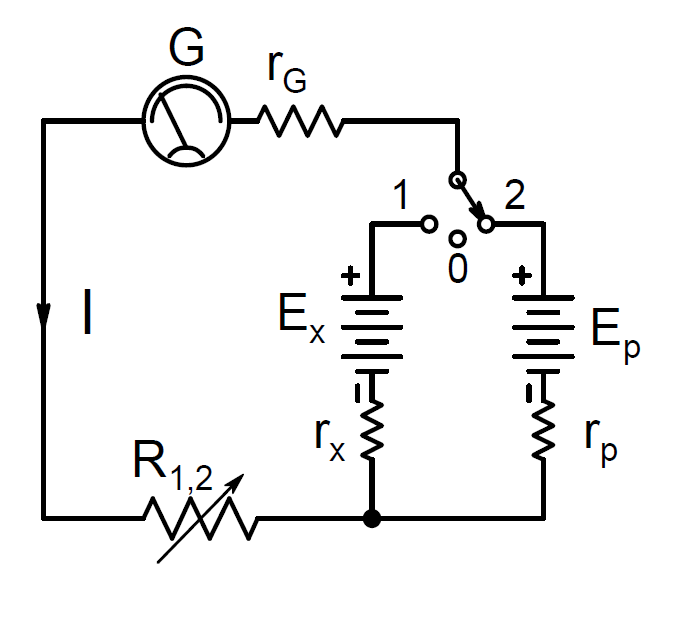
\includegraphics[width=0.5\linewidth]{ImagenesTema4/7}
	\label{fig:7}
\end{figure}
Cuando eso ocurre se cumple que:
\[\frac{E_x}{E_p}=\frac{r_x+r_G+R_1}{r_p+r_G+R_2}\]
La principal ventaja de este método es que no es necesario emplear una fuente de alimentación auxiliar. No obstante es necesario conocer las resistencias internas y que las corrientes no sean demasiado elevadas para que no alteren las f.e.m.s.

\subsubsection{Método de compensación.}
Se basa en compensar por separado la tensión patrón y la desconocido mediante una resistencia externa hasta obtener un cero de corriente en el galvanómetro. Cabe recalcar que la resistencia $R_{Aj}$ se emplea solo para ajustar la corriente.
\begin{figure}[H]
	\centering
	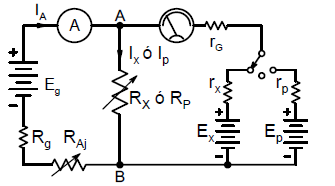
\includegraphics[width=0.5\linewidth]{ImagenesTema4/8}
	\label{fig:8}
\end{figure}
Por tanto:
\[I_x\cdot R_x=E_x\rightarrow I_G=0\rightarrow I_x=I_{A1}\]
\[I_p\cdot R_p=E_p\rightarrow I_G=0\rightarrow I_p=I_{A2}\]
\[\frac{E_x}{E_p}=\frac{I_x\cdot R_x}{I_p \cdot R_p}\]
En función de que parámetros se mantienen constantes se obtienen los siguientes métodos (aunque un parámetro no intervenga a nivel de cálculo si lo hace a nivel de incertidumbre):
\begin{itemize}
	\item Método de Dubois-Raymond: corriente constante.
\begin{figure}[H]
	\begin{minipage}{0.7\textwidth}
		\begin{figure}[H]
			\centering
			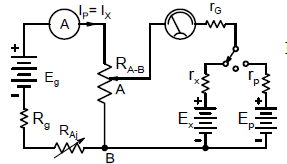
\includegraphics[width=0.7\linewidth]{ImagenesTema4/9}
			\label{fig:9}
		\end{figure}\textbf{}	
	\end{minipage}
	\begin{minipage}{0.2\textwidth}
		\[E_x=E_p\frac{R_x}{R_p}\]
	\end{minipage}
\end{figure}	
	\item Método de Poggendorf: resistencia constante.
	\begin{figure}[H]
		\begin{minipage}{0.7\textwidth}
			\begin{figure}[H]
				\centering
				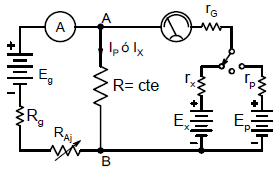
\includegraphics[width=0.7\linewidth]{ImagenesTema4/10}
				\label{fig:9}
			\end{figure}\textbf{}	
		\end{minipage}
		\begin{minipage}{0.2\textwidth}
			\[E_x=E_p\frac{I_x}{I_p}\]
		\end{minipage}
	\end{figure}	
	\item Método mixto: potenciómetro de Feussner.
	\begin{figure}[H]
		\begin{minipage}{0.5\textwidth}
			\begin{figure}[H]
				\centering
				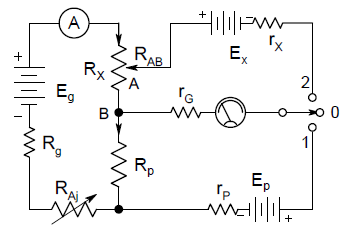
\includegraphics[width=0.7\linewidth]{ImagenesTema4/11}
				\label{fig:9}
			\end{figure}\textbf{}	
		\end{minipage}
		\begin{minipage}{0.5\textwidth}
			En este método combinado también se busca obtener el cero en el galvanómetro. Para ello, se realiza mediante los siguientes pasos:
			\begin{enumerate}
				\item Se ajusta $R_{AJ}$ en la posición 1 hasta que se obtiene un cero.
				\item Se ajusta $R_{AB}$ en la posición 2 hasta que se obtienen un cero.
			\end{enumerate}
			Una vez ajustados estos valores se cumple que:
			\[E_x=E_p\frac{R_{AB}}{R_P}\]
			Donde a la vista de la ecuación se puede observar como hay menos fuentes de incertidumbre.
		\end{minipage}
	\end{figure}
\end{itemize}
\subsection{Puente de Wheatstone para medida de resistencia.}
Es un método de cero donde mediante el ajuste de resistencias se obtiene el valor de otras.
\begin{figure}[H]
	\begin{minipage}{0.5\textwidth}
		\begin{figure}[H]
			\centering
			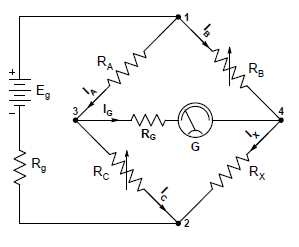
\includegraphics[width=0.7\linewidth]{ImagenesTema4/12}
			\label{fig:9}
		\end{figure}\textbf{}	
	\end{minipage}
	\begin{minipage}{0.5\textwidth}
	Como la corriente por el galvanómetro es nula:
	\[V_{13}=V_{14}\rightarrow I_A\cdot R_A =I_B \cdot R_B\]
	\[V_{32}=V_{42}\rightarrow I_A\cdot R_C =I_B \cdot R_x\]
	\[\frac{R_A}{R_C}=\frac{R_B}{R_x}\rightarrow R_x=\frac{R_B \cdot R_C}{R_A}\]
	\end{minipage}
\end{figure}

\subsubsection{Causas de incertidumbre.}
\begin{itemize}
	\item F.e.m.s en las uniones entre diferentes metales.
	\item Resistencias de contacto y de conductores.
	\item Tolerancias de las resistencias patrón.
	\item Resolución del galvanómetro.
	\item Sensibilidad del puente.
\end{itemize}
De estas causas las dos primeras solo afectan a resistencias de pequeño valor y la principal fuente de incertidumbre son las resistencias patrón.
\subsubsection{Método de sustitución.}
Se ajustan las resistencias $R_B$ y $R_C$ hasta lograr un cero en el detector. Una vez obtenida se sustituye por una resistencia variable calibrada y se ajusta nuevamente hasta obtener el cero en el detector. De esta manera, la única fuente de incertidumbre es $R_{AJ}$.

\begin{figure}[H]
	\centering
	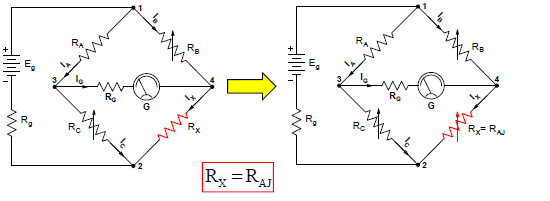
\includegraphics[width=0.7\linewidth]{ImagenesTema4/13}
	\label{fig:13}
\end{figure}



\subsubsection{Método del falso cero.}
Es un método empleado para medir la resistencia interna de un galvanómetro. Cuando el puente está en equilibrio como no circula corriente por la rama central se sabe que esta en equilibrio si la lectura del galvanómetro no cambia con el interruptor abierto o cerrado.
\begin{figure}[H]
	\begin{minipage}{0.5\textwidth}
		\begin{figure}[H]
			\centering
			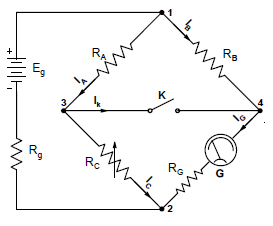
\includegraphics[width=0.7\linewidth]{ImagenesTema4/15}
			\label{fig:9}
		\end{figure}\textbf{}	
	\end{minipage}
	\begin{minipage}{0.5\textwidth}
		\[R_G=\frac{R_B\cdot R_C}{R_A}\]
	\end{minipage}
\end{figure}

\subsubsection{Puente límite.}
Es un circuito donde en función de la desviación del galvanómetro se puede conocer si una resistencia X esta dentro de tolerancias.
\begin{figure}[H]
	\centering
	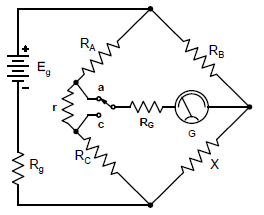
\includegraphics[width=0.35\linewidth]{ImagenesTema4/16}
	\label{fig:16}
\end{figure}


\subsubsection{Análisis de sensibilidad.}
Se entiende por sensibilidad la capacidad
para detectar los pequeños
cambios que se producen en
la condición de equilibrio
cuando se modifica alguna resistencia. Cuanto mayor sea la respuesta a esos cambios mayor
será la sensibilidad del puente y, por tanto, mayor su
capacidad para detectarlos.

\begin{figure}[H]
	\centering
	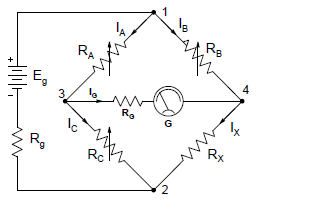
\includegraphics[width=0.5\linewidth]{ImagenesTema4/17}

	\label{fig:17}
\end{figure}
En equilibrio:
\[U_{34}=0\rightarrow I_A=I_C \ y \ I_B=I_x \rightarrow \frac{I_A \cdot R_A}{I_A \cdot R_C}=\frac{I_B \cdot R_B}{I_B \cdot R_x}\rightarrow r=\frac{R_A}{ R_C}=\frac{R_B}{R_x}\]
Suponiendo que cambia una resistencia:
\[R'_C=R_C+\Delta R_C \rightarrow U_{34}\ne 0\]
Reescribiendo las ecuaciones:
\[R'_C=R_C+\Delta R_C=R_C(1+\delta_R)\]
\[U'_{34}=U_{34}+\Delta U_{34}=\Delta U_{34}\]
No obstante como $\Delta R_C << R_C$ se puede considerar que las corrientes y tensiones permanecen prácticamente constantes. Escribiendo las ecuaciones de las tensiones y corrientes:
\[\Delta U_{34}=-I'_A\cdot R_A+I'_B\cdot R_B\]
\[I'_A \approx \frac{U_{12}}{R_A+R'_C}\]
\[I'_B\approx \frac{U_{12}}{R_B+R_x}\]
\[\Delta U_{34}\approx - \frac{R_A\cdot U_{12}}{R_A+R'_C}+\frac{R_B\cdot U_{12}}{R_B+R_x}\]
Expresándolo por unidad:
\[\delta_U=\frac{\Delta U_{34}}{U_{12}}= - \frac{R_A}{R_A+R_C(1+\delta_R)}+\frac{R_B}{R_B+R_x}\] 
Teniendo en cuenta la condición de equilibrio:
\[r=\frac{R_A}{ R_C}=\frac{R_B}{R_x}\rightarrow
\delta_U=  \frac{R_B \cdot R_C \cdot \delta_R}
{\left[R_A+R_C(1+\delta_R)\right]\cdot \left(R_B+R_x\right)}
\]
Como $\delta_R << 1 $
\[\delta_U\approx  \frac{R_B \cdot R_C \cdot \delta_R}
{\left(R_A+R_C\right)\cdot \left(R_B+R_x\right)}\]
Reescribiendo la ecuación anterior y teniendo en cuenta la relación $r$:
\[\delta_U\approx \delta_R \frac{R_C}{R_A+R_C}  \frac{R_B}{R_B+R_x}=\delta_R \frac{1}{1+r}\frac{r}{1+r}=\delta_R \frac{r}{\left(1+r\right)^2}\]
De esta manera, se define la sensibilidad por unidad como:
\[\sigma_{U/R}=\frac{\delta_U}{\delta_R}=\frac{r}{\left(1+r\right)^2}\]
\[\sigma_{V/\Omega}=\frac{\Delta U_{34}}{\Delta R_C}=\frac{r}{\left(1+r\right)^2}\frac{U_{12}}{R_C} \left[\frac{V}{\Omega}\right]\]
El punto de máxima sensibilidad:
\[\frac{\partial \sigma_{U/R}}{\partial r}=0=\frac{1-r}{\left(1+r\right)^3}\rightarrow r=1\]
Visto este valor, la máxima sensibilidad se tiene cuando:
\[r=1=\frac{R_A}{R_C}=\frac{R_B}{R_x}\]
Con el valor de:
\[\sigma_{max}=\frac{1}{4}\]
Con esta conclusión, si se invirtiera la posición de la alimentación como el equilibrio no se modifica la máxima sensibilidad se obtiene cuando todas las resistencias son iguales.
\begin{figure}[H]
	\centering
	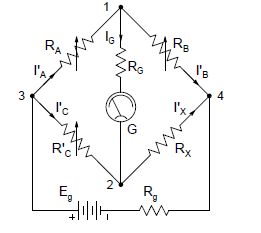
\includegraphics[width=0.5\linewidth]{ImagenesTema4/18}
	\label{fig:18}
\end{figure}

Por otro lado, se define la sensibilidad del detector como el cambio en la resistencia $R_x$ cuando se desvía del punto de equilibrio el detector.
\[\sigma_{R/U}=\frac{1}{\sigma_{U/R}}=\frac{\delta_R}{\delta_U}=\frac{\left(1+r\right)^2}{r}\]
Conocer este valor, permite reajustar el valor de la resistencia desconocida cuando no es posible alcanzar el cero por la falta de resolución en las resistencias ajustables.

\[\\\]

En la condición de mínimo se cumple que:
\[\frac{\partial \sigma_{R/U}}{\partial r}=0=\frac{r^2-1}{r^2}\rightarrow r=1\]
Por tanto, el mínimo error cometido es:
\[\sigma_{min}=4\]

Conocer la sensibilidad, permite:
\begin{enumerate}
	\item Obtener $R_x$ cuando no se puede alcanzar el cero: se basa en interpolar entre los valores que dan lugar a una lectura positiva y a otra negativa.
	\[\sigma_{\Omega/V}=\frac{\Delta R_C}{\Delta U_{34}}=\frac{R''_C-R'_C}{U''_{34}-U'_{34}}\]
	\[R_x=R'_x+\sigma_{\Omega/V} \cdot -U'_{34}=R''_x+\sigma_{\Omega/V} \cdot -U''_{34}\]
	\item Obtener la componente de incertidumbre asociada a la resolución del detector: la incertidumbre del aparato viene dada por su clase y el redondeo que se aplique a su lectura. Por tanto, al pasar estos valores a ohmios se obtiene una componente de tipo B con distribución
	 rectangular.
	 \[U_{RX}=\sigma_{\Omega/V}\cdot U_G\]
\end{enumerate}
\subsection{Puente de Kelvin-Thomson.}
Es un puente diseñado para medir resistencias de bajo valor. Este puente a diferencia de otros puentes suministra una corriente muy elevada. Como $R_{CC}$ normalmente es una barra de cobre de gran sección a efectos prácticos su resistencia es nula.
\begin{figure}[H]
	\centering
	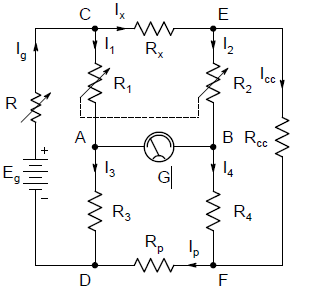
\includegraphics[width=0.5\linewidth]{ImagenesTema4/14}
	\label{fig:14}
\end{figure}
En el equilibrio:
\[U_{AB}=0\rightarrow \left\{ \begin{matrix}
	U_{CA} = U_{CB} \rightarrow I_1 \cdot R_1=I_x \cdot R_x+I_2\cdot R_2\\
	U_{AD}= U_{BD} \rightarrow I_3 \cdot R_3=I_4 \cdot R_4+I_p\cdot R_p
\end{matrix}\right.\]
En estas condiciones:
\[I_x=I_p \ \ \ \ I_1=I_3 \ \ \ \ I_2=I_4\]
Reordenando y operando se obtiene:
\[\frac{R_x}{R_p}=\frac{R_1\left(I_1  -I_2 \frac{R_2}{R_1}\right)  }{R_3\left(I_1  -I_2 \frac{R_4}{R_3}\right)}\]
Si se cumple la siguiente condición:
\[\frac{R_2}{R_1}=\frac{R_4}{R_3}\]
Entonces se cumple que:
\[R_x=\frac{R_1}{R_3}R_p\]
La suposición de que $R_{cc}=0$ no es rigurosamente cierta. No obstante si las resistencias $R_1$, $R_2$, $R_3$ y $R_4$ son mucho mayores a la resistencia patrón y la desconocida la aproximación es válido. Además, como los cocientes deben mantenerse constantes, $R_1$ y $R_2$ deben regularse a la vez.